% Requires:
% \usetikzlibrary{calc}
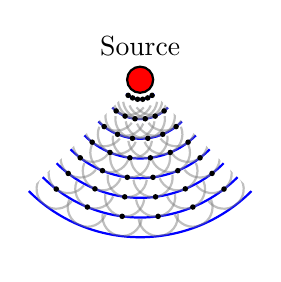
\begin{tikzpicture}
  % Primary Source
  \node[circle,draw,fill=red,thick,minimum size=0.3cm,label=above:Source] (source) at (0,0) {};

  % Primary Spherical Wavefronts
  \foreach \r in {0.25,0.5,0.75,1.0,1.25,1.5,1.75,2.0} {
    \draw[thick,blue] (source) ++(225:\r) arc (225:315:\r);
  }

  % Secondary Sources and Wavelets
  \path[clip] (source) -- ++(225:2) arc (225:315:2) -- (source);
  \foreach \r in {0.25,0.5,0.75,1.0,1.25,1.5,1.75} {
    % Centered 6 sources (spaced by 15 degrees, inset by 7.5 degrees from the edges)
    \foreach \a in {232.5, 247.5, 262.5, 277.5, 292.5, 307.5} {
      % Secondary source dot (made slightly smaller to reduce clutter since there are many)
      \fill[black] (\a:\r) circle (1pt);

      % Secondary wavelet
      \draw[thick,gray,opacity=0.5] (\a:\r) ++(\a-90:0.25) arc (\a-90:\a+90:0.25);
    }
  }
\end{tikzpicture}
